\documentclass[11pt]{article}
\usepackage[a4paper,margin=2cm]{geometry}
\usepackage[T1]{fontenc}
\usepackage{amsmath,amssymb}
\usepackage{graphicx}
\usepackage{booktabs}
\usepackage{subcaption}
\usepackage{caption}
\usepackage{microtype}
\usepackage{enumitem}
\usepackage{titlesec}
\usepackage[hidelinks]{hyperref}
\usepackage{xcolor}

\captionsetup{font=small,labelfont=bf,skip=3pt}
\setlist[itemize]{nosep,leftmargin=1.4em,topsep=1pt}
\titleformat{\section}{\normalfont\large\bfseries}{}{0pt}{}
\titlespacing*{\section}{0pt}{1.3ex plus .2ex}{0.6ex}
\setlength{\parindent}{0pt}\setlength{\parskip}{2.5pt}
\tolerance=2000 \emergencystretch=3em \hbadness=2000
\usepackage[htt]{hyphenat}
\hypersetup{colorlinks=true,urlcolor=blue!55!black,linkcolor=blue!55!black}

\newcommand{\wb}[1]{\href{https://wandb.ai/sichengma0514-university-of-cambridge/a8-grpo/runs/#1}{\texttt{#1}}}
\newcommand{\axv}[2]{\href{https://arxiv.org/abs/#1}{#2}}
\newcommand{\code}[1]{\texttt{#1}}

\begin{document}
\begin{center}
  {\Large\bfseries Part I --- GRPO Finetuning of \texttt{gemma-3-1b-it} on GSM8K}\\[3pt]
  {Multi-Agent Systems and Agentic AI --- Practical Examination}\\[5pt]
  {\small Team \textbf{chmawa} (sm3035, bc654, zw499)\quad$\cdot$\quad written individually by Zixuan Wang (zw499)}\\[3pt]
  {\small\itshape Jointly owned (shared team work): the v6e-1 TPU, the seven shared GRPO runs (\texttt{bdbugenj} and R0--R5), and the code repository.
  All prose, figure selection and interpretation below are my own.}\\[3pt]
  {\small Code: \href{https://github.com/wdk0082/a8-grpo}{\texttt{github.com/wdk0082/a8-grpo}} \emph{(to be ported to GitLab for submission)}\;$\mid$\;
  W\&B: \href{https://wandb.ai/sichengma0514-university-of-cambridge/a8-grpo}{\texttt{a8-grpo}}\;$\mid$\;
  \axv{2402.03300}{GRPO}, \axv{2503.14476}{DAPO}, \axv{2106.09685}{LoRA}, \href{https://huggingface.co/datasets/openai/gsm8k}{GSM8K}}
\end{center}
\vspace{1pt}\hrule\vspace{4pt}

\section*{I.1\quad Reproducing the baseline}
\textbf{(i) The run.} Shared baseline run (\wb{bdbugenj}): upstream commit
\href{https://github.com/borisbolliet/tpu-2026}{\texttt{borisbolliet/tpu-2026@77c5a67}}, unmodified \code{config.py},
full \textbf{3364} GRPO steps (one epoch), \textbf{4\,h\,43\,m} wall-clock on \code{v6e-1}.

\textbf{(ii) Accuracy.} GSM8K \emph{test} split (materialised from TFDS, shuffle seed 42, $n{=}64$, greedy, exact numeric match).
Base \code{gemma-3-1b-it}: \textbf{51.6\%}; LoRA checkpoint \textbf{28.1\%} at its best \emph{surviving} step (2000; \code{bdbugenj}'s earlier, better checkpoints were pruned) and \textbf{3.1\%} at step 3364.
The baseline \emph{over-optimises}: exact-match correctness falls $52\!\to\!28\!\to\!6\!\to\!3$\% across steps $0/2000/3000/3364$ while the
format-shaping reward saturates (it reward-hacks the template). At $n{=}64$ the CI is $\pm12$\,pt, so we firm the base figure to
\textbf{47.4\%} on the full 1319-example test in I.3.

\textbf{(iii) Training curves.} Fig.~\ref{fig:rewardkl} (grey = baseline): mean reward $\bar r$ peaks $\approx$\,step 450 then declines, and
$\mathrm{KL}(\pi_\theta\Vert\pi_{\mathrm{ref}})$ rises $0.16\!\to\!{\sim}0.5$ with late spikes --- the textbook over-optimisation arc.

\textbf{Baseline patches} (as-shipped fixes; full diff: \code{tpu-2026\_our\_changes.patch} in repo).
(1) \code{run\_tmux.sh} hard-coded a foreign home path; (2) the W\&B entity defaulted to a third party --- redirected to \code{a8-grpo};
(3) \code{evaluate.py} built a fresh $B{=}0$ LoRA and never restored a checkpoint, so it could only score \emph{base} --- we added Orbax
\code{--step}/\code{--ckpt-dir} LoRA restore; (4) TFDS's gsm8k builder crashes under protobuf 7.x once JAX imports, so we pre-materialise
the seed-42 test split (\code{prepare\_test\_tfds.py}) and added an HF \code{datasets} fallback.

\section*{I.2\quad Understanding the baseline}
\textbf{(a) Policies \& trainable parameters.} $\pi_\theta$ is the LoRA-adapted policy: frozen \code{gemma-3-1b-it} weights plus low-rank
adapters $\Delta W{=}BA$; \textbf{only $A,B$ are trainable} (the base is frozen). $\pi_{\mathrm{old}}$ is the policy that generated the current
rollouts --- with \code{NUM\_ITERATIONS} $\mu{=}1$ there is one gradient step per rollout batch, so $\pi_{\mathrm{old}}{=}\pi_\theta$ at the update.
$\pi_{\mathrm{ref}}$ is the frozen initial policy for the KL penalty; LoRA initialises $B{=}0$, so $\pi_\theta{=}\pi_{\mathrm{ref}}$ exactly at step 0.

\textbf{(b) Group size \& estimator.} $K{=}$\code{NUM\_GENERATIONS}$=2$. Tunix uses \code{advantage\_estimator='grpo'}: the \textbf{standard}
group-mean, std-normalised advantage $\hat A_i{=}(r_i-\bar r)/\sigma_r$ with $\bar r,\sigma_r$ over all $K$ samples \emph{including} $i$ --- \emph{not}
leave-one-out.

\textbf{(c) Shaping vs.\ correctness rewards.} Shaping: \code{match\_format\_exactly} and \code{match\_format\_approximately} (reward the
\code{<reasoning>}/\code{<answer>} template). True correctness: \code{check\_answer} and \code{check\_numbers} (extracted number vs.\ gold).
With the correctness reward \emph{alone}, an early policy is almost never numerically right, so every sample in a group scores $\approx 0$:
within-group $\sigma_r\!\to\!0$ and $\hat A_i{=}(r_i-\bar r)/\sigma_r$ has no signal (an $\varepsilon$ in the denominator averts a literal $0/0$) --- degenerate groups, no gradient. The shaping terms give
differently-formatted samples different rewards, restoring $\sigma_r>0$ and a usable advantage that bootstraps learning (the same
$\sigma_r\!\to\!0$ degeneracy analysed in I.4 Q1).

\textbf{(d) Clipped surrogate \& $\epsilon$.} The PPO-style clip lives in Tunix's \code{GRPOLearner} (module \code{tunix.rl}), in its clipped policy-gradient loss: it forms a
\textbf{per-token} ratio $\rho_t{=}\pi_\theta(a_t)/\pi_{\mathrm{old}}(a_t)$ and optimises $\min\!\big(\rho_t\hat A,\ \mathrm{clip}(\rho_t,1{-}\epsilon,1{+}\epsilon)\hat A\big)$,
with $\epsilon{=}$\code{EPSILON}$=0.2$. Two deviations from the lecture form: (i) the ratio is \textbf{per-token}, not per-sequence; (ii) at
$\mu{=}1$, $\pi_{\mathrm{old}}{=}\pi_\theta\Rightarrow\rho_t\equiv1$, so the clip is \textbf{dormant} in the baseline (it engages only for $\mu>1$).

\section*{I.3\quad Improving on the baseline}
\textbf{Modification \& motivation.} The baseline over-optimises at $K{=}2$. The theory of I.4 Q1 gives the GRPO gradient variance
$\operatorname{Var}(\hat g)=K^{-2}\sum_i(h_i-\bar h)(h_i-\bar h)^\top=O(1/K)$, with effective sample size $K_{\mathrm{eff}}\!\propto\!K$: a larger
group directly lowers the variance of the gradient estimate $\hat g$. We therefore take \textbf{group size $G$} (the $K$ of I.2(b) and the theory) as the primary lever and run a controlled
$\beta\times G$ \textbf{2$\times$2} (KL-penalty weight $\times$ group size) to separate it from the KL leash:
R4$(G2,\beta0)$, R0$(G2,\beta.08$; baseline re-run$)$, R3b$(G8,\beta0)$, R5$(G8,\beta.08)$ --- plus single-axis controls R1$(\beta{=}0.3)$ and
R2$(+\text{soft length penalty})$, for \textbf{six full runs}. All share data (HF GSM8K, seed 42), eval, horizon (3364 steps) and a seed-matched
rollout RNG (\code{PRNGKey(0)}); only the named knob changes per run. R0 re-runs the baseline config with \emph{dense} checkpoints, so its best-val
$46.7\%$ recovers the peak that \code{bdbugenj}'s pruning hid behind I.1's $28.1\%$.

\begin{table}[t]
\centering\small
\caption{Held-out accuracy on the \emph{full} GSM8K test ($n{=}1319$; HF and TFDS differ only in seed-42 ordering, so at full $n$ the I.1$\to$I.3 source switch is immaterial), greedy/exact-match, $\pm$95\% bootstrap CI.
Last column: \emph{paired} bootstrap $\Delta$ vs.\ base over the shared prompts (\code{paired\_ci.py}).
$\ast$ = paired 95\% CI excludes 0; $\dagger$ = collapse. R1$(G2,\beta.3)$ and R2$(G2,+\text{len})$ fell \emph{below} base
(R1 best 37.2 / final 0.0; R2 best 32.8 / final 40.6) --- clean negative results.}
\label{tab:acc}
\begin{tabular}{llrrr}
\toprule
Model & $(G,\beta)$, step & Acc.\,(\%) & 95\% CI & $\Delta$ base (paired) \\
\midrule
Base \code{gemma-3-1b-it} & --- & 47.4 & 44.7--50.0 & --- \\
R0 (baseline re-run) & $(2,.08)$ best 700 & 46.7 & 44.0--49.4 & $-0.7$\ \,n.s. \\
R0 & $(2,.08)$ final 3364 & 6.2 & 4.9--7.5 & $-41.2^{\dagger}$ \\
R4 & $(2,0)$ best 1300 & 52.8 & 50.1--55.5 & $+5.4^{\ast}$ \\
R4 & $(2,0)$ final 3364 & 48.6 & 45.9--51.3 & $+1.2$\ \,n.s. \\
\textbf{R3b} & $(8,0)$ best 1000 & 55.7 & 53.0--58.2 & $+8.3^{\ast}$ \\
\textbf{R3b} & $(8,0)$ \textbf{final 3364} & \textbf{57.2} & 54.6--59.9 & $+9.9^{\ast}$ \\
R5 & $(8,.08)$ best 1300 & 53.4 & 50.7--56.2 & $+6.1^{\ast}$ \\
R5 & $(8,.08)$ final 3364 & 55.6 & 52.8--58.2 & $+8.2^{\ast}$ \\
\bottomrule
\end{tabular}
\end{table}

\begin{figure}[t]
\centering
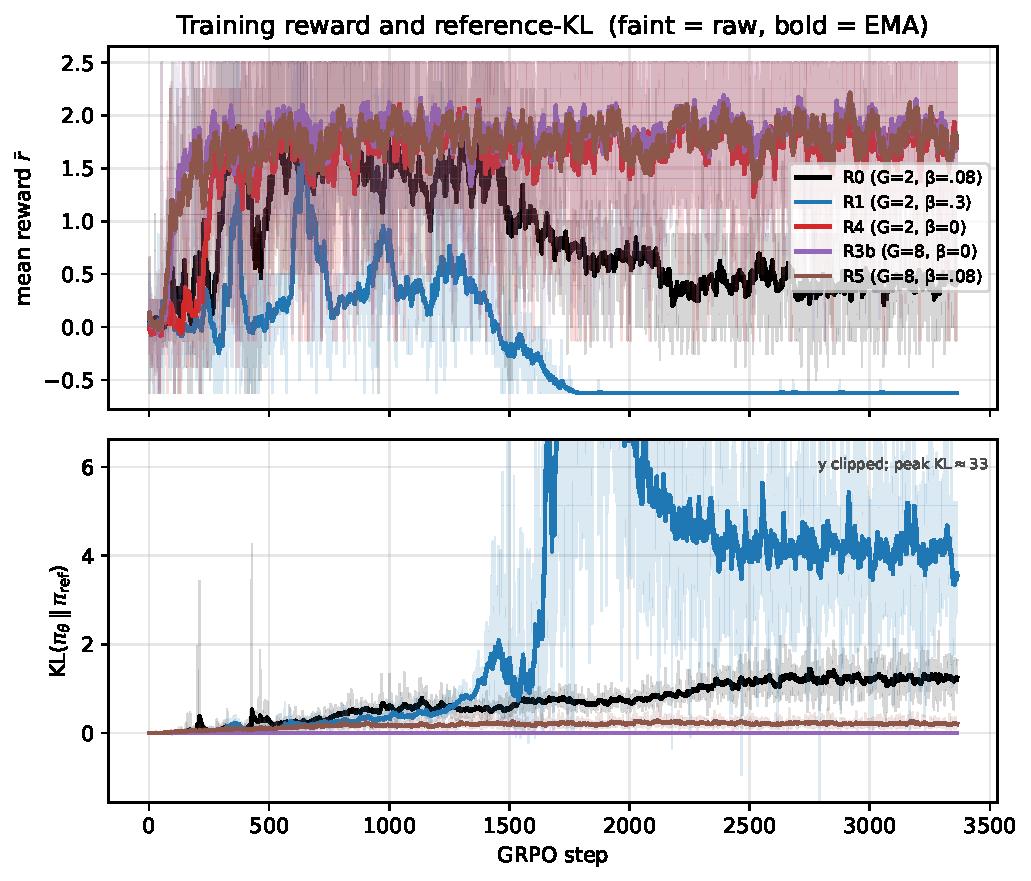
\includegraphics[width=0.86\linewidth]{F1_reward_kl.pdf}
\caption{Mean training reward $\bar r$ (top) and $\mathrm{KL}(\pi_\theta\Vert\pi_{\mathrm{ref}})$ (bottom) vs.\ GRPO step, baseline and all
variants on shared axes. Baseline/R0/R1 over-optimise (reward peaks then collapses; KL spikes); the $G{=}8$ runs (R3b, R5) and R4 stay stable.}
\label{fig:rewardkl}
\end{figure}

\begin{figure}[t]
\centering
\begin{subfigure}{0.49\linewidth}\centering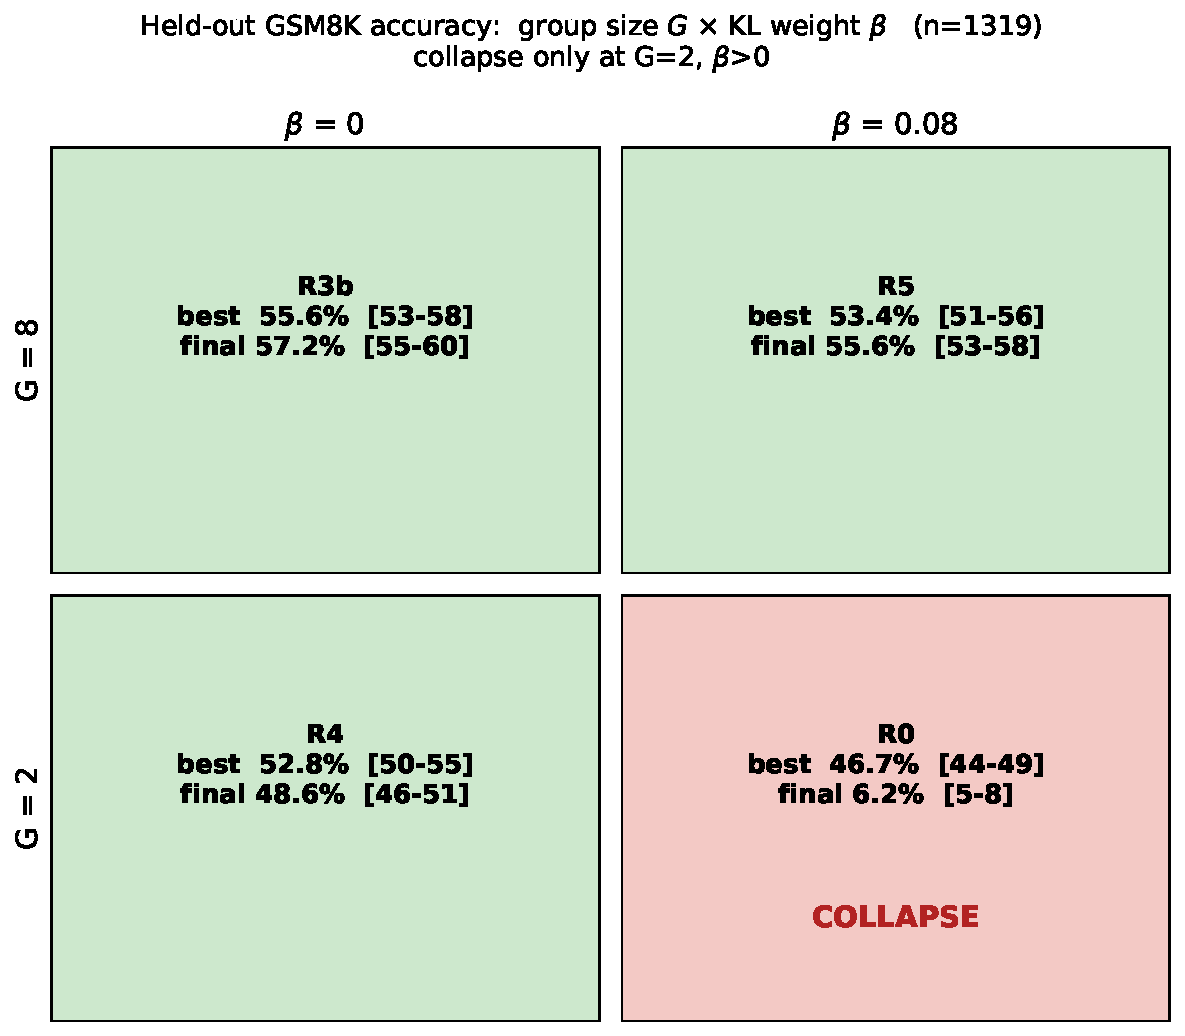
\includegraphics[width=\linewidth]{F4_2x2_GxB.pdf}\caption{$\beta\times G$ 2$\times$2 (best/final acc).}\label{fig:2x2}\end{subfigure}\hfill
\begin{subfigure}{0.49\linewidth}\centering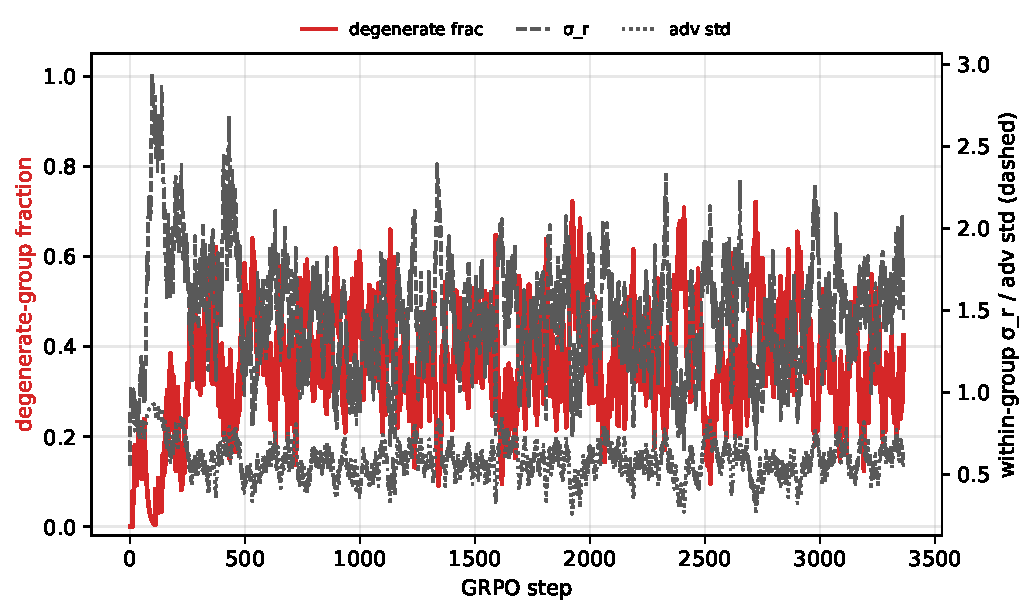
\includegraphics[width=\linewidth]{S3_group_degeneracy.pdf}\caption{Group degeneracy at $G{=}8$.}\label{fig:diag}\end{subfigure}
\caption{\emph{Left:} accuracy by $(G,\beta)$ --- collapse occurs \emph{only} at $G{=}2,\beta{>}0$ (R0). \emph{Right:} the diagnostic --- at $G{=}8$ about a
third of groups are degenerate (all-$K$ rewards equal) yet $\sigma_r$ holds $\approx1.5$ (steady, not $\to0$).}
\end{figure}

We report \textbf{(a)} held-out accuracy (Table~\ref{tab:acc}), \textbf{(b)} mean reward and KL for all runs on shared axes (Fig.~\ref{fig:rewardkl}), and \textbf{(c)} a diagnostic for a known GRPO failure mode --- group degeneracy at $G{=}8$ (Fig.~\ref{fig:diag}).

\textbf{(d) Findings vs.\ theory.} \emph{$G{=}8$ is the winning intervention.} Both $G{=}8$ runs beat base --- R3b $+9.9$, R5 $+8.2$\,pp, paired CIs
excluding 0 --- and each beats its matched $G{=}2$ run (R3b$-$R4 $=+8.6$\,pp at final; R5$-$R0 $=+49$\,pp). \textbf{R3b ($G{=}8,\beta{=}0$) is the best
model at 57.2\%.} The 2$\times$2 (Fig.~\ref{fig:2x2}) localises the failure: \emph{the collapse is confined to the $G{=}2,\beta{>}0$ corner} (R0 final
6.2\%, R1 0\%), while the \emph{same} $\beta{=}0.08$ at $G{=}8$ (R5) is stable, and at $G{=}8$ the KL weight is statistically irrelevant
(R3b vs.\ R5: $+1.7$\,pp, n.s.). Furthermore \emph{over-optimisation is itself a $G{=}2$ phenomenon}: $G{=}2$ peaks at best-val then degrades
(R4 $52.8\!\to\!48.6$; R0 collapses), whereas \textbf{$G{=}8$ improves monotonically to the final step} (final $>$ best). This is precisely the I.4 Q1
mechanism: larger $K$ shrinks $\operatorname{Var}(\hat g)$, so updates are smoother --- the policy neither reward-hacks into R0's format-only
collapse nor (once $\beta{>}0$) trips the $\exp(\log\text{-ratio})$ KL-estimator instability behind R1's blow-up.

\emph{Contradicted prediction.} We predicted an over-optimising baseline would need a \emph{tighter} KL leash. The opposite held: raising $\beta$ to
$0.3$ (R1) collapsed \emph{faster} (0\%), and removing the KL term entirely (R4, $\beta{=}0$) was fine --- the cure was variance reduction (group size),
not regularisation, echoing DAPO's removal of the KL term for long-output RL. The diagnostic (Fig.~\ref{fig:diag}) shows the cost of
$G{=}8$: $\approx\!\tfrac13$ of groups are degenerate (all-$K$-equal $\Rightarrow$ zero advantage), the $K_{\mathrm{eff}}$/dead-group issue of I.4 Q1 and
the target of DAPO's Dynamic Sampling --- yet the net effect of more rollouts is still $+8$--$10$\,pp. R1 and R2 fell below base (Table~\ref{tab:acc}),
honest negative results that further support variance, not extra shaping or a stronger leash, as the operative lever.

\clearpage
\section*{I.4\quad GRPO theory --- written questions (40 marks)}

\subsection*{I.4.1 Group-mean normalisation}

Let
\[
\bar h=\frac{1}{K}\sum_{i=1}^K h_i.
\]

\paragraph{(i)}
Since $\mathbb{E}[r_i]=\mathbb{E}[\bar r]=\mu$,
\[
\mathbb{E}[\hat A_i]
=
\frac{\mathbb{E}[r_i-\bar r]}{\sigma}
=0.
\]
Therefore
\[
\boxed{\mathbb{E}[X_i]=0},
\qquad
\boxed{\mathbb{E}[\hat g]=0}.
\]
Here the responses are conditioned on and treated as fixed, while the artificial
reward noise is independent of them. In the usual policy-gradient problem the
responses are sampled from the policy and their rewards depend on the sampled
responses, so the policy gradient need not vanish.

\paragraph{(ii)}
The common random term is the sample mean $\bar r$, appearing in every
\[
X_i=\frac{h_i}{\sigma}(r_i-\bar r).
\]
For $i\neq j$,
\begin{align*}
\operatorname{Cov}(r_i-\bar r,r_j-\bar r)
&=
\operatorname{Cov}(r_i,r_j)
-\operatorname{Cov}(r_i,\bar r)
-\operatorname{Cov}(\bar r,r_j)
+\operatorname{Var}(\bar r)\\
&=
0-\frac{\sigma^2}{K}-\frac{\sigma^2}{K}
+\frac{\sigma^2}{K}\\
&=
-\frac{\sigma^2}{K}.
\end{align*}
Hence
\[
\boxed{
\operatorname{Cov}(X_i,X_j)
=
-\frac{1}{K}h_i h_j^\top,
\qquad i\neq j.
}
\]
More precisely, the scalar covariance of the centred rewards is negative; the
cross-covariance matrix is a negative scalar multiple of $h_i h_j^\top$.
The negative dependence follows from the exact constraint
\[
\sum_{i=1}^K(r_i-\bar r)=0:
\]
if one centred reward increases, the others must collectively decrease.

\paragraph{(iii)}
For $i=j$,
\[
\operatorname{Var}(r_i-\bar r)
=
\sigma^2-\frac{\sigma^2}{K},
\]
and therefore
\[
\operatorname{Var}(X_i)
=
\left(1-\frac{1}{K}\right)h_i h_i^\top.
\]
Using all diagonal and cross-covariance terms,
\begin{align*}
\operatorname{Var}(\hat g)
&=
\frac{1}{K^2}
\sum_{i,j=1}^K
\operatorname{Cov}(X_i,X_j)\\
&=
\frac{1}{K^2}
\left[
\sum_{i=1}^K h_i h_i^\top
-\frac{1}{K}
\left(\sum_{i=1}^K h_i\right)
\left(\sum_{j=1}^K h_j\right)^\top
\right].
\end{align*}
Equivalently,
\[
\boxed{
\operatorname{Var}(\hat g)
=
\frac{1}{K^2}
\sum_{i=1}^K
(h_i-\bar h)(h_i-\bar h)^\top.
}
\]
By contrast, the mean of $K$ independent copies of $X_1$ would have covariance
\[
\operatorname{Var}_{\mathrm{iid}}(\hat g)
=
\frac{1}{K}\operatorname{Var}(X_1)
=
\frac{1}{K}
\left(1-\frac{1}{K}\right)h_1h_1^\top.
\]

Since these are matrix-valued variances, there is no canonical scalar effective
sample size. For a direction $u\in\mathbb{R}^d$ with
$u^\top\operatorname{Var}(\hat g)u>0$, define
\[
K_{\mathrm{eff}}(u)
=
\frac{
u^\top\operatorname{Var}(X_1)u
}{
u^\top\operatorname{Var}(\hat g)u
}.
\]
Then
\[
\boxed{
K_{\mathrm{eff}}(u)
=
\frac{
K^2\left(1-\frac{1}{K}\right)(u^\top h_1)^2
}{
\sum_{i=1}^K
\left(u^\top(h_i-\bar h)\right)^2
}.
}
\]
This definition gives $K_{\mathrm{eff}}(u)=K$ for the mean of $K$ genuinely
independent copies of $X_1$.

If the empirical directional dispersion
\[
\frac{1}{K}\sum_{i=1}^K
\left(u^\top(h_i-\bar h)\right)^2
\]
converges to a positive constant, then $K_{\mathrm{eff}}(u)=\Theta(K)$.
If all scores are collinear, $h_i=c_i v$, then
\[
\operatorname{Var}(\hat g)
=
\frac{vv^\top}{K^2}
\sum_{i=1}^K(c_i-\bar c)^2.
\]
Thus only variation in the coefficients $c_i$ contributes. In particular, if
all $h_i$ are identical, then
\[
\hat g
=
\frac{h_1}{K}\sum_{i=1}^K\hat A_i
=0
\]
for every reward realisation, so $\operatorname{Var}(\hat g)=0$ and the
directional effective sample size is formally infinite.


\subsection*{I.4.2 KL-regularised policy update}

\paragraph{(i)}
The objective is
\[
F(\pi)
=
\sum_a\pi(a)A_t(a)
-\frac{1}{\eta}
\sum_a\pi(a)\log\frac{\pi(a)}{\pi_t(a)}.
\]
Introducing a Lagrange multiplier $\lambda$ for $\sum_a\pi(a)=1$, stationarity
on the support of $\pi_t$ gives
\[
A_t(a)
-\frac{1}{\eta}
\left(
\log\frac{\pi(a)}{\pi_t(a)}+1
\right)
+\lambda=0.
\]
Consequently,
\[
\boxed{
\pi_{t+1}(a)
=
\frac{\pi_t(a)\exp(\eta A_t(a))}
{\sum_b\pi_t(b)\exp(\eta A_t(b))}
}.
\]
Actions outside the support of $\pi_t$ remain assigned zero probability. The
objective is strictly concave on this support, so the optimiser is unique,
assuming the normalising constant is finite.

For small $\eta$,
\[
\pi_{t+1}(a)
=
\pi_t(a)
\left[
1+\eta
\left(
A_t(a)-\mathbb{E}_{\pi_t}[A_t]
\right)
\right]
+O(\eta^2),
\]
so $\eta$ controls the update size. Large $\eta$ places increasingly more mass
on high-advantage actions.

\paragraph{(ii)}
For the true advantage of $\pi_t$,
\[
J(\pi_t)
=
\mathbb{E}_{a\sim\pi_t}[A^{\pi_t}(a)]
=0.
\]
The regularised objective evaluated at $\pi_t$ is also zero. Since
$\pi_{t+1}$ maximises it,
\[
J(\pi_{t+1})
-\frac{1}{\eta}
\operatorname{KL}(\pi_{t+1}\Vert\pi_t)
\geq 0.
\]
It follows that
\[
\boxed{
J(\pi_{t+1})
\geq
\frac{1}{\eta}
\operatorname{KL}(\pi_{t+1}\Vert\pi_t)
\geq 0
=
J(\pi_t).
}
\]
Thus the update guarantees monotone improvement in the scalar performance
measure defined in the question.

In neural-network GRPO the guarantee may fail because the exact advantage is
replaced by a noisy finite-sample estimate and the maximisation is replaced by
a finite number of stochastic-gradient steps in a restricted parametric policy
class. The clipped GRPO objective is also not identical to the exact
KL-regularised objective above.

\paragraph{(iii)}
For one sample, write
\[
\ell(\rho,\hat A)
=
\min\left(
\rho\hat A,
\operatorname{clip}(\rho,1-\epsilon,1+\epsilon)\hat A
\right).
\]
Equivalently,
\[
\ell(\rho,\hat A)
=
\begin{cases}
\hat A\min(\rho,1+\epsilon), & \hat A\geq 0,\\[2mm]
\hat A\max(\rho,1-\epsilon), & \hat A<0.
\end{cases}
\]
Thus, for a positive advantage, the objective gives no further incentive to
increase the ratio above $1+\epsilon$. For a negative advantage, it gives no
further incentive to reduce the ratio below $1-\epsilon$.

This is not a hard constraint
\[
\rho\in[1-\epsilon,1+\epsilon].
\]
Other samples can still move the ratio outside this interval. In contrast, a
constraint
\[
\operatorname{KL}
\bigl(
\pi_\theta(\cdot\mid q)
\Vert
\pi_{\mathrm{old}}(\cdot\mid q)
\bigr)
\leq\delta
\]
is a joint distribution-level constraint coupling all actions. PPO clipping is
samplewise and advantage-dependent, does not directly constrain unsampled
actions, and does not guarantee that the joint KL divergence is small.


\subsection*{I.4.3 Mixture proposal and importance weighting}

Write
\[
p(a)=\pi_{\mathrm{old}}(a\mid q),
\qquad
u(a)=\pi_{\mathrm{unif}}(a\mid q),
\qquad
m(a)=(1-\alpha)p(a)+\alpha u(a),
\]
and let
\[
s_\theta(a)=\nabla_\theta\log\pi_\theta(a\mid q).
\]
For the population analysis, define
\[
V_p=\mathbb{E}_{a\sim p}[R(q,a)],
\qquad
\sigma_p^2=\operatorname{Var}_{a\sim p}[R(q,a)],
\qquad
A_p(a)=\frac{R(q,a)-V_p}{\sigma_p}.
\]

\paragraph{(i)}
The target gradient is
\[
g_p
=
\mathbb{E}_{a\sim p}[s_\theta(a)A_p(a)].
\]
Since $m(a)\geq(1-\alpha)p(a)$, the proposal has support wherever $p$ does.
The importance weight is
\[
\boxed{
w(a)
=
\frac{p(a)}{m(a)}
=
\frac{
\pi_{\mathrm{old}}(a\mid q)
}{
(1-\alpha)\pi_{\mathrm{old}}(a\mid q)
+\alpha\pi_{\mathrm{unif}}(a\mid q)
}.
}
\]
Therefore
\[
g_p
=
\mathbb{E}_{a\sim m}
\left[
w(a)s_\theta(a)A_p(a)
\right],
\]
and an importance-corrected estimator is
\[
\boxed{
\hat g_{\mathrm{mix}}
=
\frac{1}{K}
\sum_{i=1}^K
w_i s_\theta(a_i)\hat A_i^{(p)},
\qquad
w_i=w(a_i),
}
\]
where $\hat A_i^{(p)}$ must estimate the old-policy advantage rather than the
mixture-policy advantage.

\paragraph{(ii)}
As $\alpha\to0$,
\[
m(a)\to p(a),
\qquad
w(a)\to1.
\]
Moreover, the reweighted old-policy moment estimates given below reduce to the
ordinary empirical moments. Hence, for the same realised actions,
\[
\boxed{
\hat g_{\mathrm{mix}}\longrightarrow\hat g_{\mathrm{GRPO}}.
}
\]

\paragraph{(iii-a)}
By linearity of expectation,
\[
\boxed{
V^{\pi_{\mathrm{mix}}}(q)
=
(1-\alpha)V^{\pi_{\mathrm{old}}}(q)
+
\alpha V^{\pi_{\mathrm{unif}}}(q).
}
\]

\paragraph{(iii-b)}
At the population level, for any deterministic baseline $b$,
\[
\mathbb{E}_{m}
\left[
w(a)s_\theta(a)(R(q,a)-b)
\right]
=
\mathbb{E}_{p}
\left[
s_\theta(a)(R(q,a)-b)
\right].
\]
In particular,
\begin{align*}
\mathbb{E}_{m}
\left[
w s_\theta(R-V^{\pi_{\mathrm{mix}}})
\right]
&=
\mathbb{E}_{p}
\left[
s_\theta(R-V^{\pi_{\mathrm{old}}})
\right]\\
&\quad+
\left(
V^{\pi_{\mathrm{old}}}
-
V^{\pi_{\mathrm{mix}}}
\right)
\mathbb{E}_{p}[s_\theta].
\end{align*}
At the policy-gradient evaluation point $\pi_\theta=p$,
\[
\mathbb{E}_{p}[s_\theta]
=
\mathbb{E}_{p}[\nabla_\theta\log p(a)]
=0,
\]
so a deterministic baseline shift alone does not bias the gradient.

However, the empirical $\bar r$ is a random function of the same group and the
empirical $\sigma_r$ is also proposal-dependent. Multiplying only the outer
gradient contribution by $w_i$ therefore does not transform mixture group
normalisation into old-policy group normalisation.

The intended empirical correction is to use weighted moments
\[
S_w=\sum_{j=1}^K w_j,
\qquad
\bar r_w
=
\frac{\sum_{j=1}^K w_jr_j}{S_w},
\]
and
\[
(\sigma_{r,w})^2
=
\frac{
\sum_{j=1}^K w_j(r_j-\bar r_w)^2
}{
S_w
}.
\]
The corresponding reweighted advantage is
\[
\boxed{
\hat A_i^{(w)}
=
\frac{r_i-\bar r_w}{\sigma_{r,w}},
}
\]
giving
\[
\boxed{
\hat g_{\mathrm{mix}}
=
\frac{1}{K}
\sum_{i=1}^K
w_i s_\theta(a_i)
\frac{r_i-\bar r_w}{\sigma_{r,w}}.
}
\]
This self-normalised estimator is consistent for the old-policy moments, but,
like ordinary same-group GRPO normalisation, it is not exactly unbiased at
finite $K$.

For a literally unbiased finite-$K$ baseline correction, one may instead use
the leave-one-out Horvitz--Thompson baseline
\[
\hat V_{p,-i}
=
\frac{1}{K-1}
\sum_{j\neq i}w_jr_j,
\qquad
\mathbb{E}[\hat V_{p,-i}]=V_p.
\]
Since $\hat V_{p,-i}$ is independent of $a_i$,
\[
\mathbb{E}_{m}
\left[
w_i s_\theta(a_i)
\frac{r_i-\hat V_{p,-i}}{\sigma_p}
\right]
=
\mathbb{E}_{p}
\left[
s_\theta(a)
\frac{R(q,a)-V_p}{\sigma_p}
\right].
\]
An estimated standard deviation must similarly be obtained independently if
literal finite-sample unbiasedness is required.

\paragraph{(iv)}
First ignore the additional randomness from estimating the baseline and
standard deviation. Let
\[
Y(a)=s_\theta(a)A_p(a),
\qquad
g_p=\mathbb{E}_{p}[Y(a)].
\]
Then
\[
\operatorname{Var}(\hat g_{\mathrm{GRPO}})
=
\frac{1}{K}
\left(
\mathbb{E}_{p}[YY^\top]-g_pg_p^\top
\right),
\]
whereas
\[
\operatorname{Var}(\hat g_{\mathrm{mix}})
=
\frac{1}{K}
\left(
\mathbb{E}_{m}[w^2YY^\top]-g_pg_p^\top
\right)
=
\frac{1}{K}
\left(
\mathbb{E}_{p}[wYY^\top]-g_pg_p^\top
\right).
\]
Therefore
\[
\boxed{
\operatorname{Var}(\hat g_{\mathrm{mix}})
-
\operatorname{Var}(\hat g_{\mathrm{GRPO}})
=
\frac{1}{K}
\mathbb{E}_{p}
\left[
(w-1)YY^\top
\right].
}
\]
There is no universal ordering between the two covariance matrices. In a
direction $v$,
\[
v^\top
\left[
\operatorname{Var}(\hat g_{\mathrm{mix}})
-
\operatorname{Var}(\hat g_{\mathrm{GRPO}})
\right]v
=
\frac{1}{K}
\mathbb{E}_{p}
\left[
(w-1)(v^\top Y)^2
\right].
\]
Moreover,
\[
w(a)-1
=
\frac{\alpha(p(a)-u(a))}{m(a)}.
\]
Thus mixing increases variance when large squared gradient contributions,
and hence large squared reward deviations, are concentrated on responses for
which $p(a)>u(a)$. Those responses are undersampled by the mixture relative to
$p$ and receive weights $w(a)>1$.

Conversely, mixing decreases variance when large reward deviations are
concentrated on responses for which $u(a)>p(a)$. The uniform component
oversamples these responses and their weights satisfy $w(a)<1$.

The change in the unweighted reward variance can also be seen directly:
\[
\operatorname{Var}_{m}(R)
=
(1-\alpha)\operatorname{Var}_{p}(R)
+
\alpha\operatorname{Var}_{u}(R)
+
\alpha(1-\alpha)(V_p-V_u)^2.
\]
Hence mixture sampling increases the raw reward variance if
\[
\operatorname{Var}_{u}(R)
+
(1-\alpha)(V_p-V_u)^2
>
\operatorname{Var}_{p}(R),
\]
and decreases it if the reverse inequality holds. Importance weighting adds
the separate $w^2$ effect described above.

\paragraph{(v-a)}
Under the stated assumption,
\[
w_i=c^T=\exp(T\log c).
\]
Since $0<c<1$, $\log c<0$, and therefore
\[
\boxed{
w_i\to0
\quad\text{exponentially fast as }T\to\infty.
}
\]
A ratio below one is typical for exploratory tokens or responses that are
unlikely under $\pi_{\mathrm{old}}$ but receive additional probability from
the uniform component, so that
$\pi_{\mathrm{mix}}>\pi_{\mathrm{old}}$. It is not implied for every token
merely by $\alpha>0$.

\paragraph{(v-b)}
Such trajectories make exponentially small contributions to the estimator.
If many sampled trajectories have collapsed weights, the estimate is
effectively based on only a small number of old-policy-like trajectories,
causing a small effective sample size and unstable estimates; the products may
also underflow numerically.

One unbiased remedy is to keep the proposal closer to the old policy, for
example by reducing $\alpha$ or enforcing the per-token log-ratio condition
\[
\left|
\log
\frac{
\pi_{\mathrm{old}}(a_t\mid q,a_{<t})
}{
\pi_{\mathrm{mix}}(a_t\mid q,a_{<t})
}
\right|
\leq\frac{\delta}{T}.
\]
Then
\[
e^{-\delta}\leq w_i\leq e^\delta,
\]
so the full-response weight cannot collapse exponentially. The trade-off is
weaker uniform exploration.

Alternatively, clipping or self-normalising the response weights reduces
variance and numerical collapse, but introduces bias.
\end{document}
